\documentclass[
  11pt,
  letterpaper,
   addpoints,
   answers
  ]{exam}

\usepackage{../exercise-preamble}

\begin{document}

\noindent
\begin{minipage}{0.47\textwidth}

\includegraphics[width=\textwidth]{../fcfm_die}
\end{minipage}
\begin{minipage}{0.53\textwidth}
\begin{center} 
\large\textbf{Electromagnetismo Aplicado} (EL3103-1) \\
\large\textbf{Clase auxiliar 7} \\
\normalsize Prof.~Benjamin Jacard H.\\
\normalsize Prof.~Aux.~Erik Saez A.
\end{center}
\end{minipage}

\section{Resumen: Líneas de transmisión y carta Smith}

Las líneas de transmisión se refieren a cualquier medio o estructura utilizada para transmitir señales eléctricas o electromagnéticas desde un punto a otro. Algunos ejemplos son:
\begin{itemize}
    \item \textbf{Microstrip}: Una forma de línea de transmisión utilizada en circuitos impresos, donde un conductor está colocado sobre un sustrato dieléctrico.
    \item \textbf{Cable Coaxial}: Consiste en un conductor central rodeado por un aislante y una malla conductora, utilizado comúnmente en sistemas de comunicación.
    \item \textbf{Líneas de Transmisión de RF}: Incluyen diversas configuraciones, como líneas de cinta, líneas coaxiales y líneas de microondas, utilizadas para transmitir señales de radiofrecuencia en sistemas de comunicación y electrónica.
    \item \textbf{Fibra Óptica}: Aunque técnicamente no es una línea de transmisión eléctrica, las señales de luz se utilizan para transmitir datos a través de fibras ópticas en sistemas de comunicación modernos.
\end{itemize}

En el curso nos centraremos en el líneas de transmisión de tipo rectangular y de las siguientes:

\begin{center}
    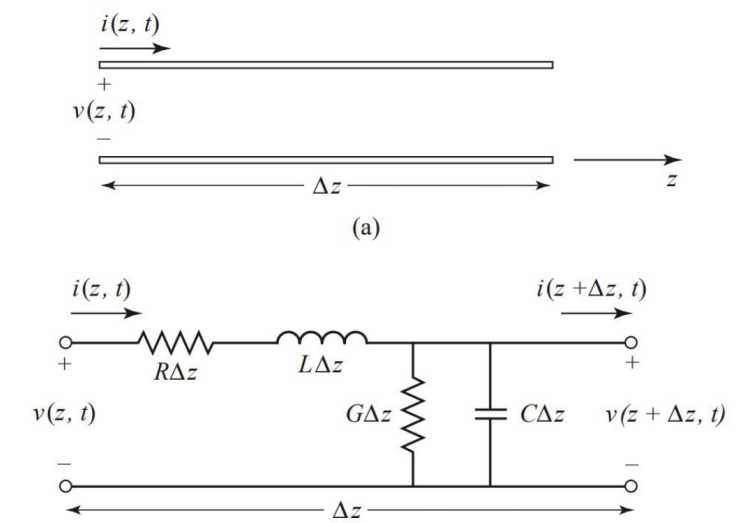
\includegraphics[width=0.5\textwidth]{Auxiliar_7_1}
\end{center}

Donde los diferentes elementos que posee la línea de transmisión representan lo siguiente:
\begin{itemize}
    \item R: Pérdida del conductor.
    \item L: Autoinductancia.
    \item G: Pérdida por el dieléctrico.
    \item C: Efecto capacitivo entre ambas líneas.
\end{itemize}

Donde las ecuaciones de voltaje y corriente vienen caracterizadas por una ecuación de onda:
\begin{align}
    \frac{\partial^2 V(z)}{\partial z^2} - \gamma^2 V(z) = 0 \tag{1} \\
    \frac{\partial^2 I(z)}{\partial z^2} - \gamma^2 I(z) = 0 \tag{2}
\end{align}

Lo que permite, mediante notación fasorial, ser expresadas como:
\begin{align}
    V(z) = V_0^+ e^{-\gamma z} + V_0^- e^{\gamma z} \tag{3} \\
    I(z) = I_0^+ e^{-\gamma z} + I_0^- e^{\gamma z} \tag{4}
\end{align}

Donde el parámetro $\gamma$ viene caracterizado por:
\begin{equation}
    \gamma = \alpha + j \beta = \sqrt{(R + j\omega L)(G + j\omega C)} \tag{5}
\end{equation}

Se logra relacionar la corriente con el voltaje como:
\begin{align}
    V(z) &= V_0^+ e^{-\gamma z} + V_0^- e^{\gamma z} \tag{6} \\
    I(z) &= \frac{1}{Z_0} \left( V_0^+ e^{-\gamma z} - V_0^- e^{\gamma z} \right) \tag{7}
\end{align}

Donde $Z_0$, el cual corresponde a la impedancia intrínseca del medio, vendrá caracterizada por:
\begin{equation}
    Z_0 = \frac{R + j\omega L}{\gamma} = \sqrt{\frac{R + j\omega L}{G + j\omega C}} \tag{8}
\end{equation}

Para el caso sin pérdidas notamos que:
\begin{equation}
    Z_0 = \sqrt{\frac{L}{C}} \tag{9}
\end{equation}

Luego, tenemos que dicha impedancia intrínseca también puede ser expresada como:
\begin{equation}
    \frac{V_0^+}{V_0^-} = Z_0 = -\frac{V_0^-}{I_0^-} \tag{10}
\end{equation}

Es importante en lo que viene entender el concepto de impedancia de entrada $Z_{in}$, que será demostrado más adelante, así como el funcionamiento de los adaptadores $\lambda/2$ y $\lambda/4$.

\subsection*{Carta de Smith}

La Carta de Smith, o Diagrama de Smith, es una herramienta gráfica utilizada en ingeniería de radiofrecuencia y diseño de líneas de transmisión. Esta carta proporciona una representación visual de las impedancias en un sistema de transmisión de radiofrecuencia. Esta se construye y se utiliza a partir de:
\begin{itemize}
    \item \textbf{Normalización de impedancias}: Normaliza las impedancias dividiendo cada valor de impedancia por la impedancia característica de la línea de transmisión utilizada. Esto crea impedancias normalizadas, que son adimensionales.
    \item \textbf{Ubicación en el Gráfico Polar}: Representa cada impedancia normalizada como un punto en el gráfico polar. La parte real se coloca en el eje horizontal (resistivo) y la parte imaginaria en el eje vertical (reactivo).
    \item \textbf{Círculos concéntricos en el gráfico}: Representan líneas de constante resistencia y reactancia normalizadas. Estos círculos ayudan a visualizar cambios en la impedancia a medida que varía la frecuencia.
    \item \textbf{Líneas radiales}: Estas líneas representan ángulos constantes y se utilizan para medir el ángulo de la impedancia normalizada desde el eje resistivo.
    \item \textbf{Movimientos generador--plano carga}: La carta Smith permite visualizar los movimientos que se realizan hacia el generador o hacia el eje, lo cual es muy útil.
\end{itemize}

La Carta de Smith se construye a partir de impedancias en lugar de admitancias debido a que es más común trabajar con impedancias en el contexto de líneas de transmisión y sistemas de radiofrecuencia. Aun así, se puede utilizar para admitancias dado que equivale a una rotación de $180^\circ$. Esta carta puede ser difícil de utilizar en un principio pero luego se vuelve intuitiva e incluso preferible por sobre otros métodos de resolución en el contexto de líneas.
\begin{center}
    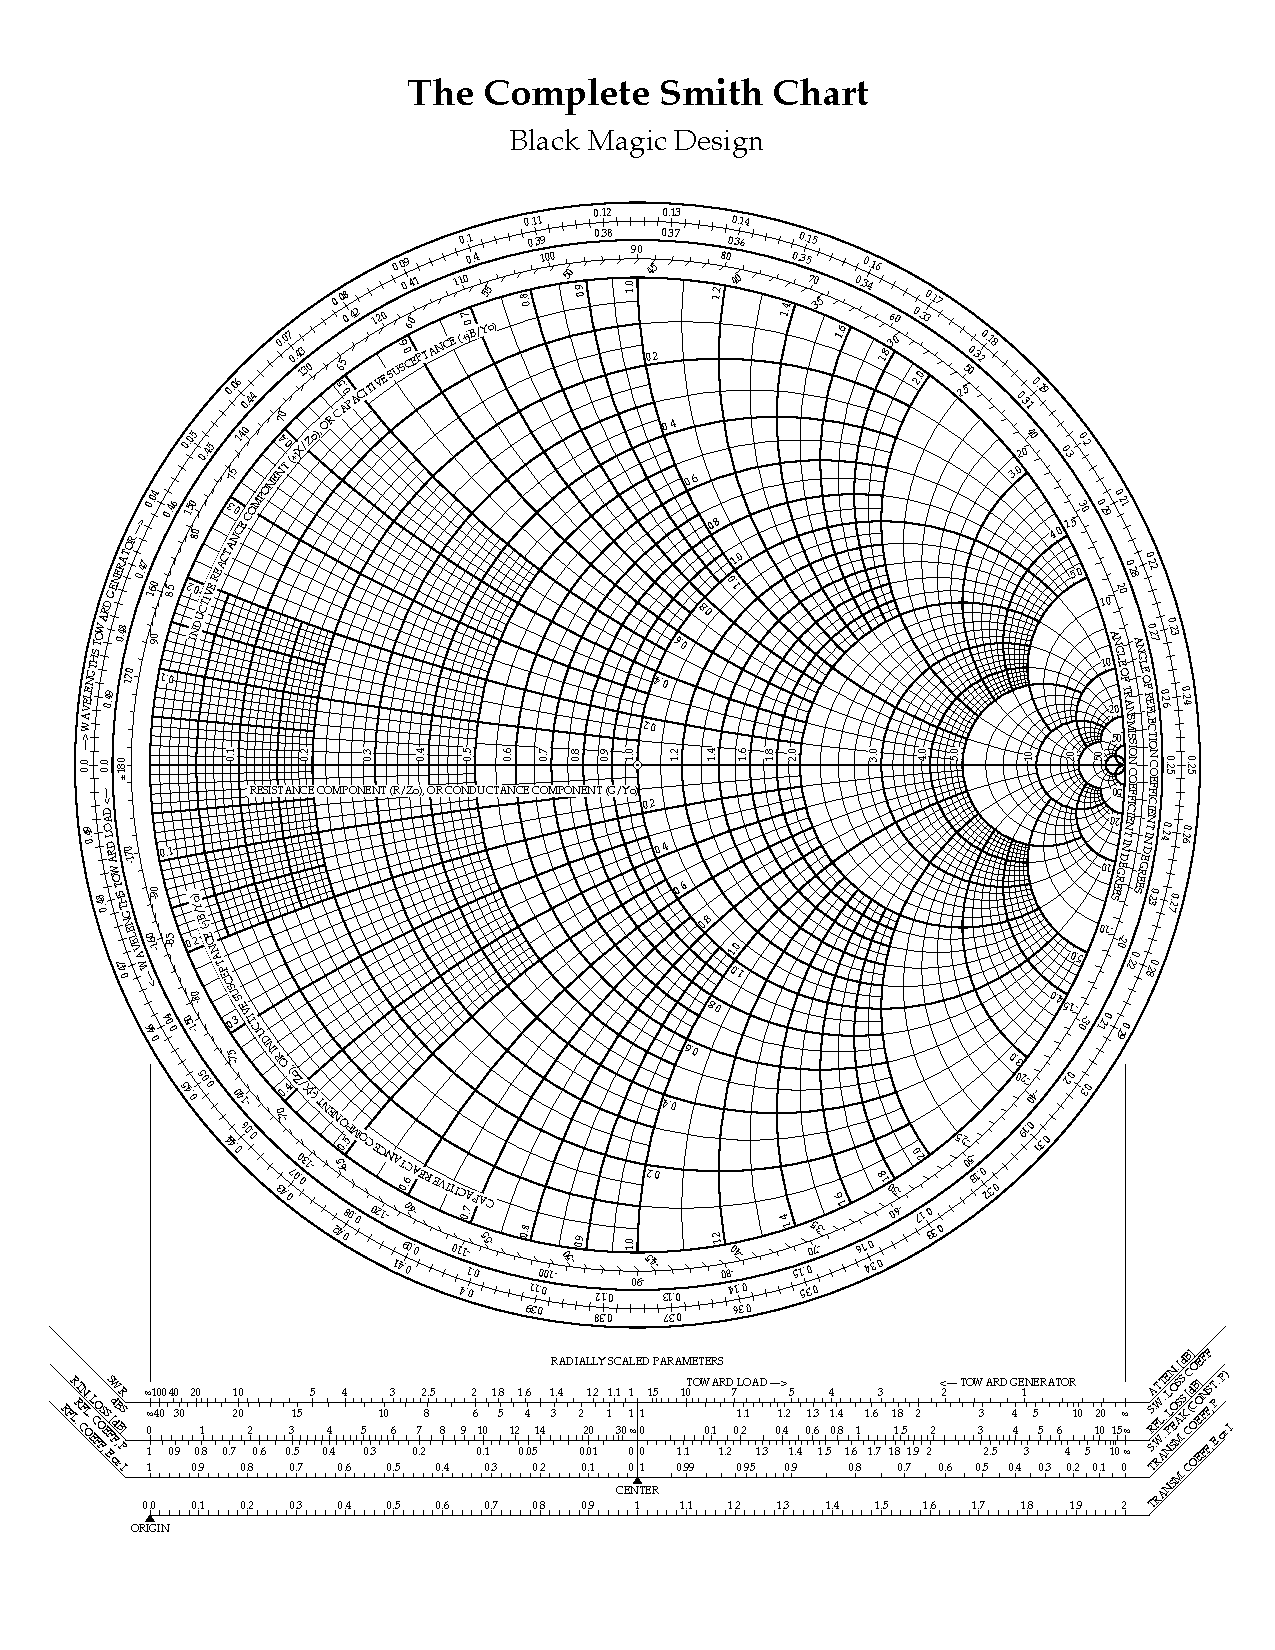
\includegraphics[width=0.7\textwidth]{SmithChart}
\end{center}

\vspace{0.5cm}
\noindent
\vspace{.85cm}
\begin{questions}
    %%%%%%%%%%%%%%%%%%%%%%%%%%%%
    \question
    \begin{enumerate}
    \item Demuestre que la impedancia de entrada de una línea sin pérdidas de largo $l$, constante de fase $\beta$ e impedancia característica $Z_c$, con una impedancia de carga $Z_L$, está dado por:
    \[
    Z_{in} = Z_c \left( \frac{Z_L + j Z_c \tan(\beta l)}{Z_c + j Z_L \tan(\beta l)} \right)
    \]
    
    \item Sea la carga un corto-circuito obtenga el $Z_{in}$ e interprete el resultado.
    
    \item Sea la carga un circuito abierto obtenga el $Z_{in}$ e interprete el resultado.
    
    \item Se busca el analizar la impedancia de entrada en la situación que $l = \lambda/2$; además interprete el resultado. Obtenga el coeficiente de reflexión de la carga.
    
    \item Se busca el analizar la impedancia de entrada en la situación que $l = \lambda/4$; además interprete el resultado. Obtenga el coeficiente de reflexión de la carga.
\end{enumerate}
  \begin{center}
        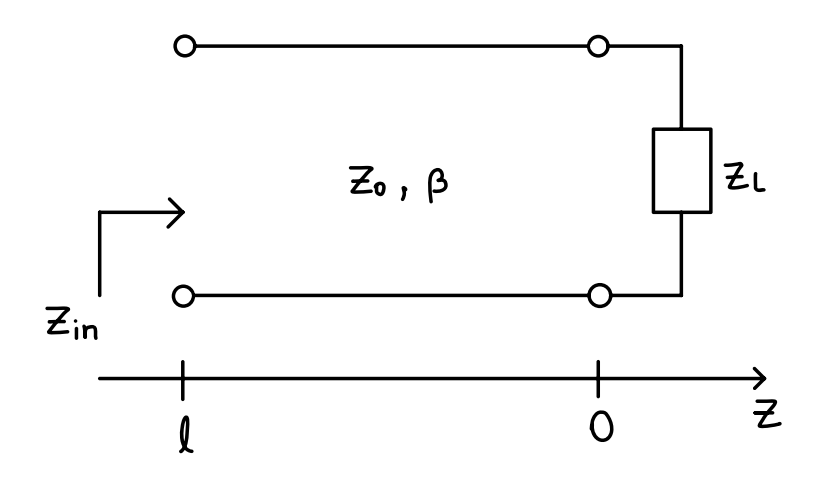
\includegraphics[width=0.5\textwidth]{Auxiliar_7_4}
        \captionof{figure}{Esquema de la linea de transmisión}
      \end{center}
    %%%%%%%%%%%%%%%%%%%%%%%%%%%
    \begin{solution}
        \begin{enumerate}
            \item Se realiza el análisis de la impedancia de entrada de una línea de transmisión terminada en una carga $Z_{l}$. Por ello, se considera la presencia tanto de una onda incidente como de una onda reflejada a lo largo de la línea de transmisión. Así, tanto la corriente como el voltaje pueden expresarse como:
\begin{align}
    V(z) &= V^{+}e^{-j\beta z} + V^{-}e^{j\beta z} \\
    I(z) &= I^{+}e^{-j\beta z} - I^{-}e^{j\beta z}
\end{align}

El valor de la impedancia para las ondas incidente y reflejada es:
\begin{align}
    \frac{V^{+}}{I^{+}} = \frac{V^{-}}{I^{-}} = Z_{c}
\end{align}

En relación al sistema de referencia, calculando voltaje y corriente en la posición de la carga (es decir, en $z=0$), se obtiene:
\begin{align}
    V(z=0) = V^{+} + V^{-} = V^{+}(1+\Gamma_{L})
\end{align}
donde se utiliza que el coeficiente de reflexión en la carga es $\Gamma_{L} = \frac{V^{-}}{V^{+}}$.

De manera análoga, la corriente en $z=0$ es:
\begin{align}
    I(z=0) &= I^{+} - I^{-} = \frac{V^{+}}{Z_{c}} - \frac{V^{-}}{Z_{c}} \\
           &= \frac{1}{Z_{c}} (V^{+} - V^{-}) \\
           &= \frac{V^{+}}{Z_{c}} (1 - \Gamma_{L})
\end{align}

Por lo tanto, la impedancia en la carga se puede calcular como:
\begin{align}
    Z_{l} = \frac{V(z=0)}{I(z=0)} = \frac{V^{+}(1+\Gamma_{L})}{\frac{V^{+}}{Z_{c}} (1-\Gamma_{L})} = \frac{Z_{c}(1+\Gamma_{L})}{1-\Gamma_{L}}
\end{align}

De aquí, despejando el coeficiente de reflexión en la carga:
\begin{align}
    Z_{l} &= \frac{Z_{c}(1+\Gamma_{L})}{1-\Gamma_{L}} \\
    Z_{l}(1-\Gamma_{L}) &= Z_{c}(1+\Gamma_{L}) \\
    Z_{l} - Z_{l}\Gamma_{L} &= Z_{c} + Z_{c}\Gamma_{L} \\
    Z_{l} - Z_{c} &= Z_{l}\Gamma_{L} + Z_{c}\Gamma_{L} \\
    Z_{l} - Z_{c} &= \Gamma_{L}(Z_{l} + Z_{c}) \\
    \Gamma_{L} &= \frac{Z_{l} - Z_{c}}{Z_{l} + Z_{c}}
\end{align}

Si se evalúa la impedancia de entrada para una distancia arbitraria $z = -l$:
\begin{align}
    Z_{in} = \frac{V(z=-l)}{I(z=-l)} = \frac{V^{+}e^{j\beta l} + V^{-}e^{-j\beta l}}{\frac{1}{Z_{c}} \left( V^{+}e^{j\beta l} - V^{-}e^{-j\beta l} \right)}
\end{align}

Dividiendo numerador y denominador por $V^{+}$:
\begin{align}
    Z_{in} = Z_{c} \left( \frac{e^{j\beta l} + \Gamma_{L} e^{-j\beta l}}{e^{j\beta l} - \Gamma_{L} e^{-j\beta l}} \right)
\end{align}

Es importante notar que el coeficiente de reflexión sigue estando \textbf{asociado a la carga} (es decir, evaluado en la carga). Reemplazando el valor obtenido anteriormente:
\begin{align}
    Z_{in} = Z_{c} \left( \frac{e^{j\beta l} + \left( \frac{Z_{l}-Z_{c}}{Z_{l}+Z_{c}} \right) e^{-j\beta l}}{e^{j\beta l} - \left( \frac{Z_{l}-Z_{c}}{Z_{l}+Z_{c}} \right) e^{-j\beta l}} \right)
\end{align}

Multiplicando numerador y denominador por $Z_{l}+Z_{c}$:
\begin{align}
    Z_{in} &= Z_{c} \left( \frac{ (Z_{l}+Z_{c}) e^{j\beta l} + (Z_{l}-Z_{c}) e^{-j\beta l} }{ (Z_{l}+Z_{c}) e^{j\beta l} - (Z_{l}-Z_{c}) e^{-j\beta l} } \right) \\
           &= Z_{c} \left( \frac{ Z_{l}(e^{j\beta l} + e^{-j\beta l}) + Z_{c}(e^{j\beta l} - e^{-j\beta l}) }{ Z_{c}(e^{j\beta l} + e^{-j\beta l}) + Z_{l}(e^{j\beta l} - e^{-j\beta l}) } \right)
\end{align}

Luego, utilizando las siguientes identidades trigonométricas:
\begin{align}
    e^{j\theta} + e^{-j\theta} = 2\cos(\theta) \\
    e^{j\theta} - e^{-j\theta} = 2j\sin(\theta)
\end{align}

Reemplazando en la ecuación anterior, se obtiene:
\begin{align}
    Z_{in} = Z_{c} \left( \frac{ Z_{l} \cdot 2\cos(\beta l) + 2j Z_{c} \sin(\beta l) }{ Z_{c} \cdot 2\cos(\beta l) + 2j Z_{l} \sin(\beta l) } \right)
\end{align}

Dividiendo numerador y denominador por $2\cos(\beta l)$:
\begin{align}
    Z_{in} = Z_{c} \left( \frac{ Z_{l} + jZ_{c} \tan(\beta l) }{ Z_{c} + jZ_{l} \tan(\beta l) } \right)
\end{align}

De este modo, se obtiene la expresión de la impedancia de entrada para una \textbf{distancia $l$ arbitraria}, una expresión fundamental en el análisis de líneas de transmisión.
        \item  Cuando la impedancia de carga es un cortocircuito, $Z_{l} = 0$, se obtiene:

\begin{center}
    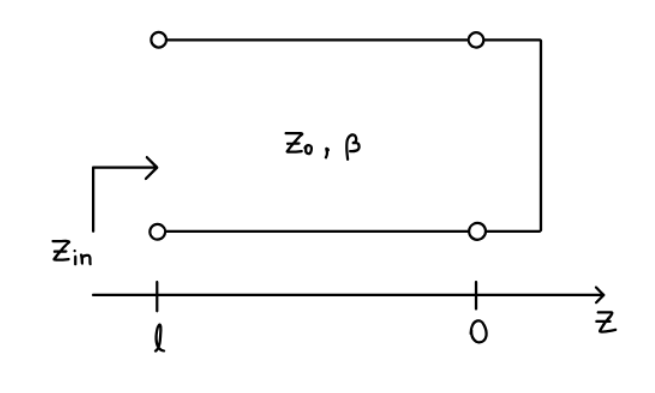
\includegraphics[width=0.45\textwidth]{Auxiliar_7_2}
\end{center}

La impedancia de entrada es:
\begin{align}
    Z_{in} &= Z_{c} \left( \frac{Z_{l} + jZ_{c} \tan(\beta l)}{Z_{c} + jZ_{l} \tan(\beta l)} \right) \\
    &= Z_{c} \left( \frac{0 + jZ_{c} \tan(\beta l)}{Z_{c} + j \cdot 0 \cdot \tan(\beta l)} \right) \\
    &= jZ_{c} \tan(\beta l)
\end{align}

Para el coeficiente de reflexión:
\begin{align}
    \Gamma_{l} = \frac{Z_{l} - Z_{c}}{Z_{l} + Z_{c}} = \frac{0 - Z_{c}}{0 + Z_{c}} = -1
\end{align}
Es decir, hay reflexión total con inversión de fase ($\pi$).


\item Cuando la carga es un circuito abierto, $Z_{l} \rightarrow \infty$:

\begin{center}
    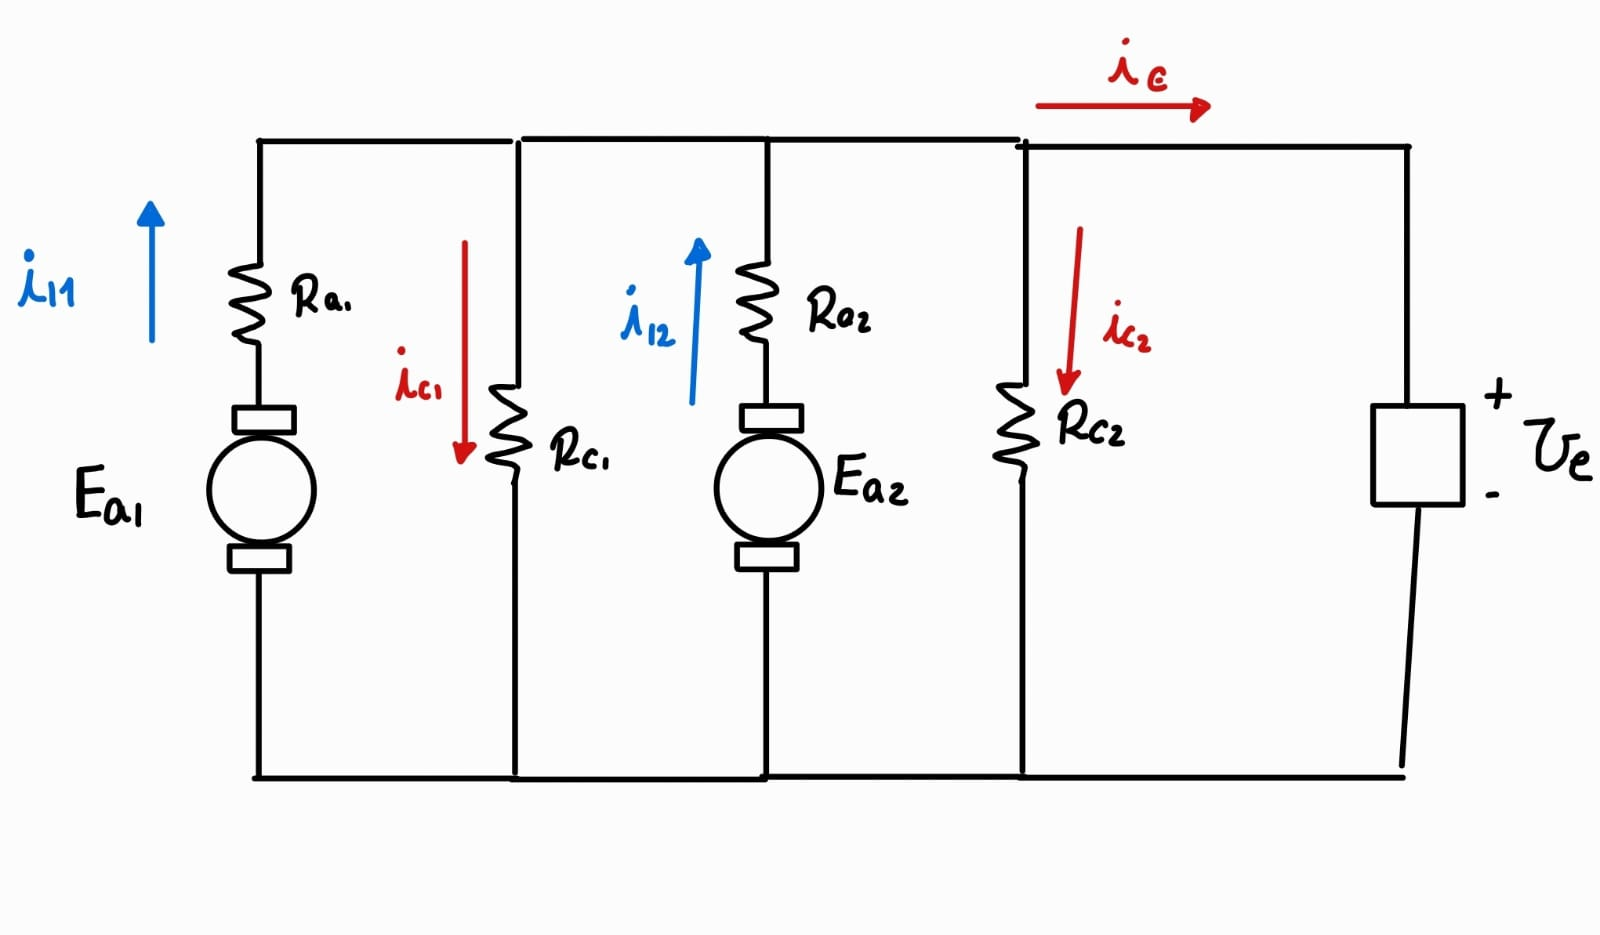
\includegraphics[width=0.45\textwidth]{Auxiliar_7_3}
\end{center}

La impedancia de entrada es:
\begin{align}
    Z_{in} &= Z_{c} \left( \frac{Z_{l} + jZ_{c} \tan(\beta l)}{Z_{c} + jZ_{l} \tan(\beta l)} \right)
\end{align}
Dividiendo numerador y denominador por $Z_{l}$ y tomando el límite $Z_{l} \to \infty$:
\begin{align}
    Z_{in} &= Z_{c} \left( \frac{1 + j \frac{Z_{c}}{Z_{l}} \tan(\beta l)}{\frac{Z_{c}}{Z_{l}} + j \tan(\beta l)} \right) \\
    &\xrightarrow{Z_{l} \to \infty} Z_{c} \left( \frac{1 + 0}{0 + j \tan(\beta l)} \right) \\
    &= - Z_{c} \cot(\beta l)
\end{align}

El coeficiente de reflexión en este caso es:
\begin{align}
    \Gamma_{l} = \frac{Z_{l} - Z_{c}}{Z_{l} + Z_{c}} \xrightarrow{Z_{l} \to \infty} 1
\end{align}
Es decir, hay reflexión total sin inversión de fase.
\item Para una longitud $l = \frac{\lambda}{2}$:
\begin{center}
    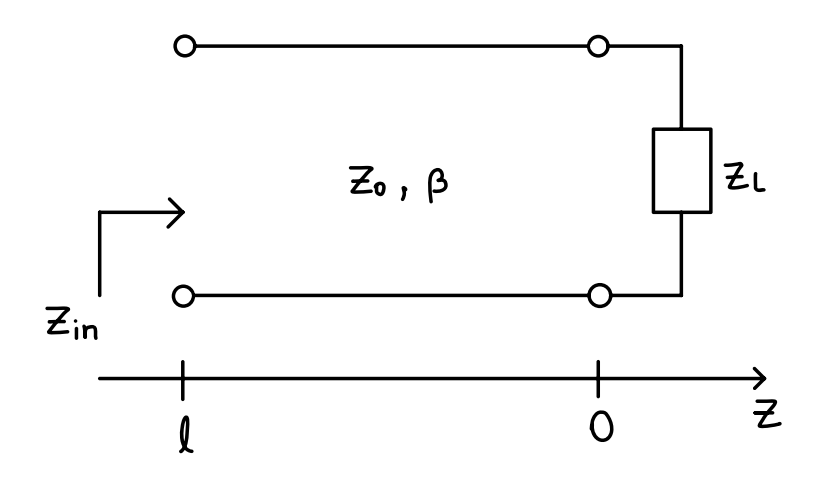
\includegraphics[width=0.45\textwidth]{Auxiliar_7_4}
\end{center}

Se tiene:
\begin{align}
    Z_{in} &= Z_{c} \left( \frac{Z_{l} + jZ_{c} \tan\left(\beta \frac{\lambda}{2}\right)}{Z_{c} + jZ_{l} \tan\left(\beta \frac{\lambda}{2}\right)} \right)
\end{align}
Recordando que $\beta = \frac{2\pi}{\lambda}$:
\begin{align}
    \beta \frac{\lambda}{2} = \frac{2\pi}{\lambda} \cdot \frac{\lambda}{2} = \pi \\
    \tan(\pi) = 0
\end{align}
Por lo tanto,
\begin{align}
    Z_{in} = Z_{c} \left( \frac{Z_{l} + jZ_{c} \cdot 0}{Z_{c} + jZ_{l} \cdot 0} \right) = Z_{c} \left( \frac{Z_{l}}{Z_{c}} \right) = Z_{l}
\end{align}

Esto muestra que la impedancia de entrada de una línea de longitud $\lambda/2$ es igual a la impedancia de carga, independientemente de la impedancia característica de la línea.
\item Para una longitud $l = \frac{\lambda}{4}$:
\begin{align}
    Z_{in} &= Z_{c} \left( \frac{Z_{l} + jZ_{c} \tan\left( \beta \frac{\lambda}{4} \right) }{Z_{c} + jZ_{l} \tan\left( \beta \frac{\lambda}{4} \right)} \right)
\end{align}
Nuevamente, usando $\beta = \frac{2\pi}{\lambda}$:
\begin{align}
    \beta \frac{\lambda}{4} = \frac{2\pi}{\lambda} \cdot \frac{\lambda}{4} = \frac{\pi}{2} \\
    \tan\left( \frac{\pi}{2} \right) \to \infty
\end{align}
Por lo tanto:
\begin{align}
    Z_{in} &\approx Z_{c} \left( \frac{jZ_{c} \cdot \infty}{jZ_{l} \cdot \infty} \right) = Z_{c} \left( \frac{Z_{c}}{Z_{l}} \right) = \frac{Z_{c}^2}{Z_{l}}
\end{align}

Esta distancia es de suma importancia y muy útil en aplicaciones de microondas, ya que permite adaptar la impedancia variando $Z_{c}$ para minimizar reflexiones en la línea.

        \end{enumerate}
    \end{solution}
    %%%%%%%%%%%%%%%%%%%%%%%%%%%%
    \question 
    Sea el valor de la carga $Z_L = 32$ y $Z_0 = 50$ (línea que viene desde el generador), obtenga el valor de la impedancia característica de la línea de adaptación ($Z_c$) para que el sistema se encuentre adaptado, además obtenga el coeficiente de reflexión e interprete el resultado obtenido. Si la impedancia tuviera una componente compleja, ¿qué podría suceder y cómo se solucionaría?

    \begin{center}
        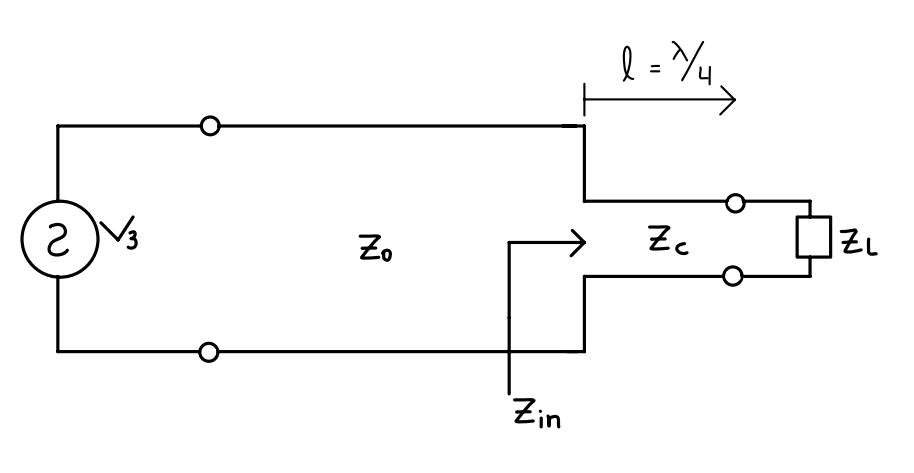
\includegraphics[width=0.5\textwidth]{Auxiliar_7_5}
        \captionof{figure}{Esquema del adaptador de adaptación}
      \end{center}
    %%%%%%%%%%%%%%%%%%%%%%%%%%%%
    \begin{solution}
         \begin{enumerate}
            \item En base al esquema visto, se tendrá la presencia de un adaptador de $\frac{\lambda}{4}$, que recordando su expresión:

\begin{equation}
    Z_{in} = Z_{c} \frac{Z_{l} + jZ_{c} \tan(\beta l)}{Z_{c} + jZ_{l} \tan(\beta l)}
    \tag{63}
\end{equation}

Se tendrá para $l = \frac{\lambda}{4}$ (\textit{distancia desde la carga a donde queremos medir la impedancia de entrada}):
\begin{align}
    Z_{in} &= Z_{c} \frac{Z_{l} + jZ_{c}\tan\left( \beta \cdot \frac{\lambda}{4} \right)}{Z_{c} + jZ_{l} \tan\left( \beta \cdot \frac{\lambda}{4} \right)} \notag\\
           &= Z_{c} \frac{Z_{l} + jZ_{c}\tan\left( \frac{\pi}{2} \right)}{Z_{c} + jZ_{l} \tan\left( \frac{\pi}{2} \right)} \notag\\
           &= \frac{Z_{c}^2}{Z_{l}}
    \tag{64}
\end{align}

Con lo que obtenemos una expresión que no depende de $\beta$ ni de otros términos, por lo que se logra obtener el $Z_{c}$ que necesitamos para una impedancia de carga $Z_{l}$, por tanto:

\begin{equation}
    Z_{c} = \sqrt{Z_{in} \cdot Z_{l}} = \sqrt{50 \cdot 32} \approx 40\,[\Omega]
    \tag{65}
\end{equation}

Esta condición impuesta es debido a que se desea una impedancia de entrada de $Z_{in} = 50\,[\Omega]$ \textit{(Para que se logre ver desde el adaptador que no existan reflexiones y la onda no presente una condición en el medio que produzca reflexiones)}. Esto da como resultado una impedancia de característica de línea de $Z_{c} \approx 40\,[\Omega]$. 

Luego, si queremos obtener el coeficiente de reflexión en donde se mide $Z_{in}$, se obtiene:

\begin{align}
    \Gamma &= \frac{Z_{0} - Z_{in}}{Z_{0} + Z_{in}} = \frac{50 - \frac{Z_{c}^2}{Z_{l}}}{50 + \frac{Z_{c}^2}{Z_{l}}} = \frac{50 - 50}{50 + 50} = 0
\end{align}

Es decir que la línea se encuentra totalmente adaptada, lo cual es óptimo ya que no tendremos las reflexiones que pueden producir inconvenientes. Se tendrá que este procedimiento es válido para impedancias con solo componente real, dado que no es posible obtener un $Z_{c} \in \mathbb{C}$ dado que no es posible implementarlo en la vida real; la solución la veremos en problemas posteriores.

         \end{enumerate}
    \end{solution}
     
    
%%%%%%%%%%%%%%%%%%%%%%%%%%%
\end{questions}
\newpage
%%%%%%%%%%%%%%%%%%%%%%%%%%%

\end{document}